\section{Theorie}
\label{sec:Theorie}

% In knapper Form sind die physikalischen Grundlagen des Versuches, des Messverfahrens, sowie sämtliche für die Auswertung erforderlichen Gleichungen darzustellen. (Keine Herleitung)

% (eventuell die Aufgaben)

% Der Versuchsaufbau: Beschreibung des Versuchs und der Funktionsweise (mit Skizze/Bild/Foto)

Wenn ein Körper deformiert wird und diese Deformation den elastischen Bereich nicht überschreitet, wird der Zusammenhang zwischen Spannung $\sigma$ und Deformationsverhältnis $\Delta L / L$ beschrieben durch das Hookesche Gesetz
\begin{equation}
    \sigma = E \frac{\Delta L}{L}.\text{\cite{V103}}
\end{equation}
Wobei $E$ der Elastizitätsmodul und somit eine Materialkonstante ist.
\begin{figure}
    \centering
    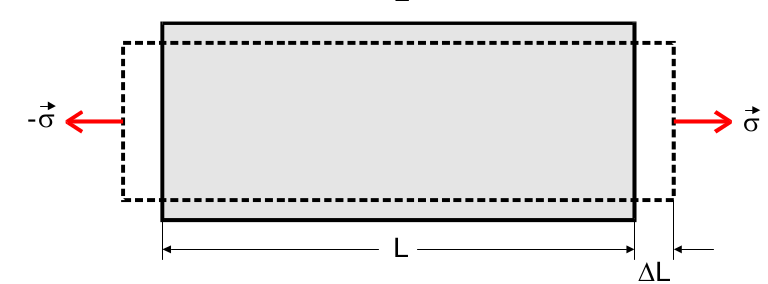
\includegraphics[width=\textwidth]{images/skizze_1.png}
    \caption{Dehnung einer stabförmigen Probe unter dem Einfluss einer Normalspannung\cite{V103}}
    \label{skizze_1}
\end{figure}

Nun kann die Biegung eines Stabes durch die Kraft $F$ auch als Dehnung angesehen werden, da eine Seite gedehnt und die andere Seite gestaucht wird. 
Zwischen diesen Seiten liegt eine Fläche, welche weder gestreckt noch gestaucht ist.
Diese Fläche nennt man die neutrale Faser.